\documentclass[12pt]{article}
\usepackage{graphicx}
\usepackage{geometry}
\usepackage{hyperref}
\usepackage{float}
\geometry{a4paper, margin=1in}
\usepackage{fancyhdr}
\pagestyle{fancy}
\fancyhf{}
\rhead{
\includegraphics[width=2cm]{img/logo.png}}
\lhead{Socio-Economic Factors \& Agricultural Pricing}
\rfoot{Page \thepage}

\begin{document}

% Custom title page
\begin{titlepage}
    \centering
    \vspace*{\fill} % Add vertical space to push the content to the middle
    
\includegraphics[width=10cm]{img/logo2.png}\\[1cm] % Adjust the path as necessary
    {\Large \textbf{Socio-Economic Factors Affecting Agricultural Pricing in Pakistan}}\\[0.5cm]
    {\large Muhammad Saad}\\[0.2cm]
    {\large \today}\\[0.5cm]
    \vspace*{\fill}
\end{titlepage}

\newpage
\tableofcontents
\newpage

\section*{Abstract}
\addcontentsline{toc}{section}{Abstract}
This report provides an in-depth analysis of the socio-economic factors affecting agricultural pricing in Pakistan, focusing on key areas such as farmer education, farm size, and family size. Utilizing data from the Agricultural Census 2010 and supplementary studies, the report examines how these factors influence agricultural productivity and economic sustainability. By understanding the demographic attributes of farmers, the distribution and size of farms, and the role of family labor, the report aims to highlight critical areas for policy intervention and strategic development. Detailed provincial breakdowns and technical insights are provided to offer a comprehensive view of the agricultural landscape in Pakistan.

\section*{Background Information}
\addcontentsline{toc}{section}{Background Information}
Agriculture is a fundamental sector in Pakistan's economy, providing employment to a significant portion of the population and contributing substantially to the country's GDP. The agricultural landscape of Pakistan is diverse, ranging from the fertile plains of Punjab and Sindh to the rugged terrains of Khyber Pakhtunkhwa (KPK) and Balochistan. This sector is characterized by various socio-economic factors that influence its productivity and pricing mechanisms.

\subsection*{Socio-Economic Factors in Agriculture}
Socio-economic factors such as education levels of farmers, farm sizes, and family sizes play critical roles in determining the efficiency and productivity of agricultural activities. Education impacts the ability of farmers to adopt new technologies and practices, while farm size influences the feasibility of mechanization and economies of scale. Family size affects labor availability and the overall socio-economic burden on agricultural households.

\subsection*{Challenges in the Agricultural Sector}
The agricultural sector in Pakistan faces several challenges, including land fragmentation, water scarcity, and limited access to modern farming technologies. Fragmentation of land, often due to inheritance practices, leads to inefficiencies in farm management. Water scarcity, particularly in arid regions like Balochistan, hampers crop yields and sustainability. Additionally, a significant portion of farmers has limited access to advanced agricultural technologies, affecting their productivity and competitiveness.

\subsection*{Importance of Policy Interventions}
Effective policy interventions are crucial to address these challenges and improve the agricultural sector's productivity. Policies aimed at land consolidation, enhancing access to education and training for farmers, and improving infrastructure can significantly impact agricultural output. Furthermore, tailored regional policies considering the unique geographical and socio-economic conditions of each province can drive sustainable agricultural development.


\section{Causes}
The variation in farmer education, family size, and farm size in Pakistan can be attributed to several interrelated factors:

\subsection*{Farmer Education}
The disparity in education levels among farmers is influenced by multiple socio-economic and cultural factors:
\begin{itemize}
    \item \textbf{Economic Constraints:} Many farming families have limited financial resources, which can restrict their ability to afford education for their children. The need for children to contribute to farm labor further reduces the likelihood of pursuing higher education.
    \item \textbf{Geographical Barriers:} Rural and remote areas often lack access to quality educational institutions, making it difficult for farmers and their families to obtain formal education.
    \item \textbf{Cultural Norms:} In some communities, cultural norms and traditional roles may prioritize agricultural work over formal education, especially for males who are expected to take over family farms.
    \item \textbf{Government Policies:} Insufficient government investment in rural education infrastructure and programs also contributes to the lower educational attainment among farmers.
\end{itemize}

\subsection*{Family Size}
Variations in family size among farmers are influenced by economic, cultural, and social factors:
\begin{itemize}
    \item \textbf{Labor Needs:} Larger families are often seen as beneficial in agricultural communities due to the increased availability of family labor for farm work. This traditional view supports higher birth rates.
    \item \textbf{Economic Security:} In agrarian societies, children are viewed as a source of economic support and security for parents in their old age, leading to larger family sizes.
    \item \textbf{Access to Healthcare:} Limited access to family planning services and healthcare in rural areas can result in higher birth rates and larger families.
\end{itemize}

\subsection*{Farm Size}
The size of farms varies due to several factors, including historical, economic, and policy influences:
\begin{itemize}
    \item \textbf{Inheritance Practices:} Traditional inheritance practices, particularly in rural areas, lead to the subdivision of land among heirs, resulting in smaller and more fragmented farms over generations.
    \item \textbf{Land Tenure Systems:} The type of land tenure and property rights systems in place can influence farm sizes. Secure land tenure encourages investment in larger farms, while insecure tenure can result in fragmented and smaller farms.
    \item \textbf{Government Policies:} Policies related to land reforms, agricultural subsidies, and rural development can impact farm sizes. Land reform policies, for instance, aim to distribute land more equitably but can also result in smaller farm sizes.
\end{itemize}

Understanding these underlying causes is essential for developing targeted interventions to address disparities in education, family size, and farm size, ultimately improving the productivity and sustainability of Pakistan's agricultural sector.

\section{Effects}
The socio-economic factors of farmer education, family size, and farm size have profound impacts on agricultural productivity and pricing in Pakistan:

\subsection*{Farmer Education}
\begin{itemize}
    \item \textbf{Adoption of Technology:} Educated farmers are more likely to adopt modern agricultural technologies and practices, leading to increased productivity and efficiency. Conversely, lower education levels hinder the adoption of these advancements, maintaining traditional and often less productive farming methods.
    \item \textbf{Access to Information:} Higher educational attainment facilitates better access to and understanding of agricultural information, enabling farmers to make informed decisions regarding crop management, pest control, and market conditions.
    \item \textbf{Economic Management:} Educated farmers are generally better at financial planning and management, which can lead to improved profitability and sustainability of their farming operations.
\end{itemize}

\subsection*{Family Size}
\begin{itemize}
    \item \textbf{Labor Supply:} Larger family sizes provide a readily available labor force, which is essential for labor-intensive farming practices. This can enhance productivity, particularly in regions where mechanization is less feasible.
    \item \textbf{Resource Allocation:} Larger families may face challenges in allocating sufficient resources, such as land and capital, among all members, potentially leading to fragmented and less efficient farming operations.
    \item \textbf{Economic Burden:} The economic burden of larger families can strain financial resources, limiting investments in farm improvements and technology adoption.
\end{itemize}

\subsection*{Farm Size}
\begin{itemize}
    \item \textbf{Economies of Scale:} Larger farms benefit from economies of scale, allowing for more efficient use of resources, reduced costs per unit of production, and increased overall productivity. Smaller farms, in contrast, often struggle with higher per unit costs and lower efficiency.
    \item \textbf{Mechanization:} Larger farms are more conducive to mechanization, which can significantly boost productivity and reduce labor costs. Smaller farms may find it challenging to justify the investment in machinery due to limited land area.
\end{itemize}

\section{Use Cases}
\subsection{South Asia}
In South Asia, particularly in Pakistan and India, the agricultural sector is characterized by small, fragmented farms and large family sizes. The limited educational attainment among farmers hampers the adoption of modern agricultural technologies. Family labor is a crucial component of farm operations, reflecting the reliance on traditional farming methods. Government initiatives focus on improving education and land consolidation to enhance productivity.

\subsection{Europe}
European agriculture benefits from higher levels of farmer education, larger average farm sizes, and advanced mechanization. The European Union's Common Agricultural Policy (CAP) provides significant subsidies and support for farmers, promoting sustainable agricultural practices and technological adoption. The high level of education among farmers facilitates efficient farm management and innovation.

\subsection{America}
In the United States and Canada, the agricultural sector is marked by very large farm sizes, high mechanization, and advanced technology use. Farmers typically have access to extensive education and training programs, which contribute to high productivity levels. Government policies provide substantial support through research, development, and subsidies, fostering a competitive and efficient agricultural industry.

\subsection{Asia}
In other parts of Asia, such as China and Japan, there is a mix of large and small farms with varying levels of mechanization. In China, significant government efforts are focused on land consolidation and improving farmer education to boost productivity. Japan's agriculture is characterized by small, intensively cultivated farms with high levels of mechanization and technology adoption, supported by government policies aimed at maintaining rural economies.

These use cases highlight the diverse agricultural landscapes and the varying impacts of socio-economic factors on productivity and sustainability across different regions. Targeted policies that address specific regional challenges and leverage strengths are essential for improving agricultural outcomes globally.

\section{Arguments Against and For}
\subsection*{Arguments For}
\begin{itemize}
    \item \textbf{Enhanced Productivity:} Addressing socio-economic factors such as education, farm size, and family size can significantly improve agricultural productivity and efficiency.
    \item \textbf{Economic Stability:} Educated farmers with access to larger, consolidated farms are better positioned to achieve economic sustainability, reducing poverty and increasing rural development.
    \item \textbf{Technological Adoption:} Improved education levels facilitate the adoption of modern agricultural technologies, leading to increased yields and better resource management.
\end{itemize}

\subsection*{Arguments Against}
\begin{itemize}
    \item \textbf{Implementation Costs:} Addressing these factors requires substantial investment in education, infrastructure, and land consolidation, which may be challenging for resource-limited governments.
    \item \textbf{Resistance to Change:} Farmers accustomed to traditional practices may resist changes, making the implementation of new policies and technologies difficult.
    \item \textbf{Equity Concerns:} Policies focusing on land consolidation and mechanization might marginalize smallholder farmers, exacerbating socio-economic inequalities.
\end{itemize}

\section{Datasets}
\subsection{Farmer's Education}
Based on the study by Yaseen et al. (2016) which provides a comparative analysis of ICT usage among farmers in Pakistan and China, the educational levels of farmers have significant implications for their ability to utilize advanced technologies in agriculture. In Pakistan, approximately \textbf{56.3\%} of farmers have received \textbf{more than 10 years of education}, potentially equipping them with the skills necessary to engage with modern farming technologies and practices. However, \textbf{43.8\%} of farmers with \textbf{less than 10 years of schooling} may face challenges in adopting such technologies due to limited literacy and numeracy skills, which are crucial for understanding and implementing new agricultural techniques.

This disparity in educational attainment among farmers can lead to significant variations in farming efficiency and productivity. Educated farmers are generally better positioned to access, interpret, and utilize agricultural information from various sources, including government advisories, agricultural apps, and market news, which are essential for making informed decisions about crop management, pest control, and the use of fertilizers and pesticides.

\subsection{Farm Size}
According to the Agricultural Census of Pakistan 2010, the total number of farms in Pakistan amounts to approximately 8.26 million, covering an area of 52.91 million acres. This gives an average farm size of 6.4 acres across the country, with a variation in average cultivated area standing at 5.2 acres per farm.

\subsubsection{Provincial Distribution}
\begin{itemize}
    \item \textbf{Khyber Pakhtunkhwa (KPK)}: Comprises 19\% of the total farms, averaging smaller farm sizes of 3.6 acres, reflecting the mountainous terrain which limits large-scale agriculture.
    \item \textbf{Punjab}: Dominates with 64\% of the farms, averaging 5.6 acres. Known for its fertile plains, Punjab facilitates intensive agriculture, contributing significantly to the national agricultural output.
    \item \textbf{Sindh}: Holds 13\% of the farms with larger average sizes of 8.8 acres, suitable for extensive crop production including major cash crops like sugarcane and wheat.
    \item \textbf{Balochistan}: Has the largest average farm size at 22.7 acres, accounting for 4\% of the total farms. The large farm size is typical of the region's pastoral and nomadic farming practices.
\end{itemize}

\subsubsection{Cultivation and Land Use}
Each province's agricultural capability is influenced by its farm size distribution, where larger farms in Balochistan face challenges such as water scarcity impacting their cultivation intensity. In contrast, Punjab and Sindh achieve higher cultivation densities due to better irrigation systems and fertile lands.

\subsubsection{Technical Implications}
\begin{itemize}
    \item \textbf{Mechanization Feasibility}: Smaller farms, especially in KPK and Punjab, struggle with the feasibility of mechanization, which could enhance productivity if farm sizes were more conducive.
    \item \textbf{Economic Sustainability}: The economic viability of smaller farms is often questioned due to higher per unit costs and lower economies of scale. Policies aimed at land consolidation could potentially address these issues.
\end{itemize}

\subsubsection{Figure: Distribution of Average Size of Farm}
\begin{figure}[H]
    \centering
    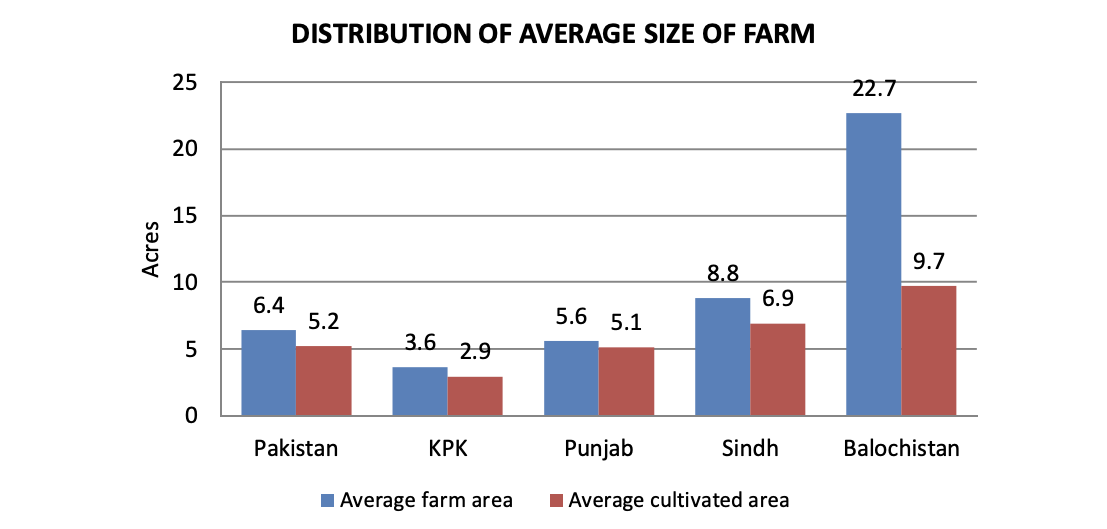
\includegraphics[width=0.8\textwidth]{img/distribution_of_farm_sizes.png}
    \caption{Distribution of average farm size by province in Pakistan.}
    \label{fig:farm_size_distribution}
\end{figure}

Strategic interventions to optimize farm sizes through land consolidation programs, tailored extension services to improve farm management practices, and enhanced access to technology could drive significant improvements in agricultural productivity across Pakistan.

\subsection{Family Size of Farmers in Pakistan}
The Agricultural Census 2010 reveals that the average family size in agricultural households across Pakistan is 7.1, which is on par with the national average household size. This suggests a strong familial workforce presence in agricultural sectors, which is pivotal for labor-intensive farming practices prevalent across the country.

\subsubsection{Provincial Breakdown}
\begin{itemize}
    \item \textbf{Punjab:}
    \begin{itemize}
        \item Average Household Size: 6.6 in agricultural households.
        \item Analysis: Punjab, being the agricultural hub of Pakistan, has a slightly lower family size in farming households compared to the national average. This reflects the intensive farming practices and a high dependency on manual labor. Despite the slightly smaller family size, Punjab's efficient use of resources and extensive irrigation systems support its robust agricultural output.
    \end{itemize}
    \item \textbf{Sindh:}
    \begin{itemize}
        \item Average Household Size: 7.5 in agricultural households.
        \item Analysis: The average family size in Sindh is larger than the national average, supporting its extensive agricultural operations, particularly in labor-intensive crops like rice and wheat. The larger family size indicates a substantial labor force within households, which is crucial for managing the high demand for labor in crop cultivation and harvesting.
    \end{itemize}
    \item \textbf{Khyber Pakhtunkhwa (KPK):}
    \begin{itemize}
        \item Average Household Size: 8.2 in agricultural households.
        \item Analysis: KPK exhibits significantly larger family sizes, which are essential for supporting agricultural activities in its rugged and mountainous terrain. The larger households provide the necessary labor pool for diverse agricultural operations, including both crop production and livestock management, adapting to the region's challenging geographic conditions.
    \end{itemize}
    \item \textbf{Balochistan:}
    \begin{itemize}
        \item Average Household Size: 9.3 in agricultural households.
        \item Analysis: Balochistan has the largest average family sizes among farmers, which is critical for managing its extensive livestock holdings and large farm sizes. The larger family units help mitigate the labor demands of vast and less densely populated agricultural lands, emphasizing the role of family labor in sustaining agricultural productivity in this arid region.
    \end{itemize}
\end{itemize}

\subsubsection{Socio-Economic Implications}
Larger family sizes in agricultural settings suggest a dependency on family labor, which, while beneficial for labor supply, also places significant economic and social demands on these households. The findings underscore the need for targeted support in educational programs, healthcare access, and agricultural subsidies to enhance the livelihoods and productivity of these communities.

\section*{Conclusion \& Opinions}
\addcontentsline{toc}{section}{Conclusion \& Opinions}
Based on the comprehensive data and analyses, several key observations and insights emerge regarding the socio-economic factors affecting agricultural productivity and pricing in Pakistan.

Firstly, the disparity in educational levels among farmers is striking. While a significant portion of farmers have more than 10 years of schooling, a considerable number still lack basic education. This educational gap presents both a challenge and an opportunity. On one hand, it highlights the immediate need for targeted educational programs to bring all farmers to a level where they can effectively utilize modern agricultural technologies. On the other hand, it underscores the potential gains in productivity and efficiency that could be realized by improving educational access and quality for farmers.

Secondly, the analysis of farm sizes reveals a fragmented agricultural landscape, particularly in Khyber Pakhtunkhwa and Punjab. Small, fragmented farms struggle with mechanization and achieving economies of scale, which hampers productivity. In contrast, larger farms in Balochistan, although facing challenges like water scarcity, have the potential to leverage economies of scale more effectively. There is a clear need for policies that encourage land consolidation and provide support for small farmers to adopt collaborative farming practices or cooperatives, enhancing their collective bargaining power and resource access.

Thirdly, the family size data paints a picture of a labor-intensive agricultural sector heavily reliant on family labor. Larger family sizes, particularly in Balochistan and KPK, provide the necessary labor for farming but also impose significant economic burdens. This dual-edged sword necessitates policies that support these large families through better healthcare, education, and economic opportunities outside of farming to reduce dependency on agriculture alone.

\newpage
\section*{References}
\addcontentsline{toc}{section}{References}
\begin{enumerate}
    \item Yaseen, Muhammad \& Xu, Shiwei \& Wen, yu \& Luqman, Muhammad \& Hassan, Sadia \& Ameen, Muhammad. (2016). Factors Inhabiting ICTs usage among Farmers: Comparative Analysis from Pakistan and China. \textit{Open Journal of Social Sciences}, 4, 287-294. doi: 10.4236/jss.2016.45031.
    \item Food and Agriculture Organization Microdata at FAO, Agricultural Census 2010, Pakistan.
    \item Pakistan Bureau of Statistics, Agricultural Census 2010 - Table 1A: Number and Area of Farms by Size of Farm. Available online: \url{https://www.pbs.gov.pk/sites/default/files/agriculture/publications/agricultural_census2010/table01a.pdf}
    \item Pakistan Bureau of Statistics, Agricultural Census 2010 - Table 8A: Number of Households and Household Members by Sex and Age and by type of Household. Available online: \url{https://www.pbs.gov.pk/sites/default/files/agriculture/publications/agricultural_census2010/table08a.pdf}.
\end{enumerate}

\end{document}
